\documentclass[conference,twocolumn]{IEEEtran}
\IEEEoverridecommandlockouts
% The preceding line is only needed to identify funding in the first footnote. If that is unneeded, please comment it out.
\usepackage{cite}
\usepackage{amsmath,amssymb,amsfonts}
\usepackage{float}
\usepackage{algorithmic}
\usepackage{graphicx}
\usepackage{textcomp}
\usepackage{authblk}
\usepackage{pifont}
\usepackage{url} 
\usepackage{pdfpages}
\usepackage{tabularx}
\usepackage{authblk}
\usepackage[utf8]{inputenc}
\usepackage{graphicx}
\graphicspath{ {figures/} }
\usepackage{array}
\def\BibTeX{{\rm B\kern-.05em{\sc i\kern-.025em b}\kern-.08em
   T\kern-.1667em\lower.7ex\hbox{E}\kern-.125emX}}
 
\pagenumbering{roman}

  
 
\begin{document}
\title{\LaTeX\ Biometrics Project Report}

\title{Digital Smile Design}
\author[1]{Ahmed Hossam}
\author[1]{Ahmed Abdelfattah }
\author[1]{Ehab Wahba }
\author[1]{Mo'men Maged}
\author[1]{Mohaned Alaa }
\author[1]{Mostafa Mahmoud}
\affil[1]{Systems and Biomedical Engineering, Cairo University}


\renewcommand\Authands{ and }

\maketitle
\pagestyle{plain}

\begin{abstract}
    Digital smile design is a unique dental treatment planning tool that strengthens a dental provider's diagnostic vision, enhances predictability, and improves communication between dental providers and their patients.
    We've designed a software solution that is easy to use for everyone. The software can detect 4 defects in a person's smile. Moreover, it provides some solutions and templates to change these defects.
    The software works with high accuracy and time effeciency compared to traditional methods.
\end{abstract}
\section{\textbf{Introduction}}
\textbf {M}any dentists use traditional methods such as \textbf{Power Point} templates to aid them in the process of smile design. 
 Such method is easy to use, accessable, and free. However, it is time consuming and provides low effeciency results.
 We've also tested the trial version of an already existing software called \textbf{Smile Designer Pro} which had a much simpler interface than Power Point templates. It can also detect the facial midline and the mouth boundaries.
 Nevertheless, is semi-automatic and requires a lot of human modifications.\\
 The presented software was designed to detect 4 defects in a smile: midline shift, discoloration, gummy smile and diastema.
 We also provided different teeth templates according to the person's facial structure.
 

\section{\textbf{Materials and Methods}}
\subsection{Facial Landmarks}
 We've collected 49 profile shots from different sources (i.e. our collegues, the internet and dentists) of smiling people.\\
 At first, we've used \textbf{Google}'s landmark facial detector API to detect certain points to crop the mouth from the face image, and determine the facial midline.
 However, it required constant internet connection and didn't provide as many points around the mouth for a smooth cropping.\\
 Finally, we used \textbf{dlib}'s facial landmarks recognition free library as it provided 68 points which are enough to crop the mouth from the image smoothly, and detect the facial midline points.
 \begin{figure}[H]
    \centering
    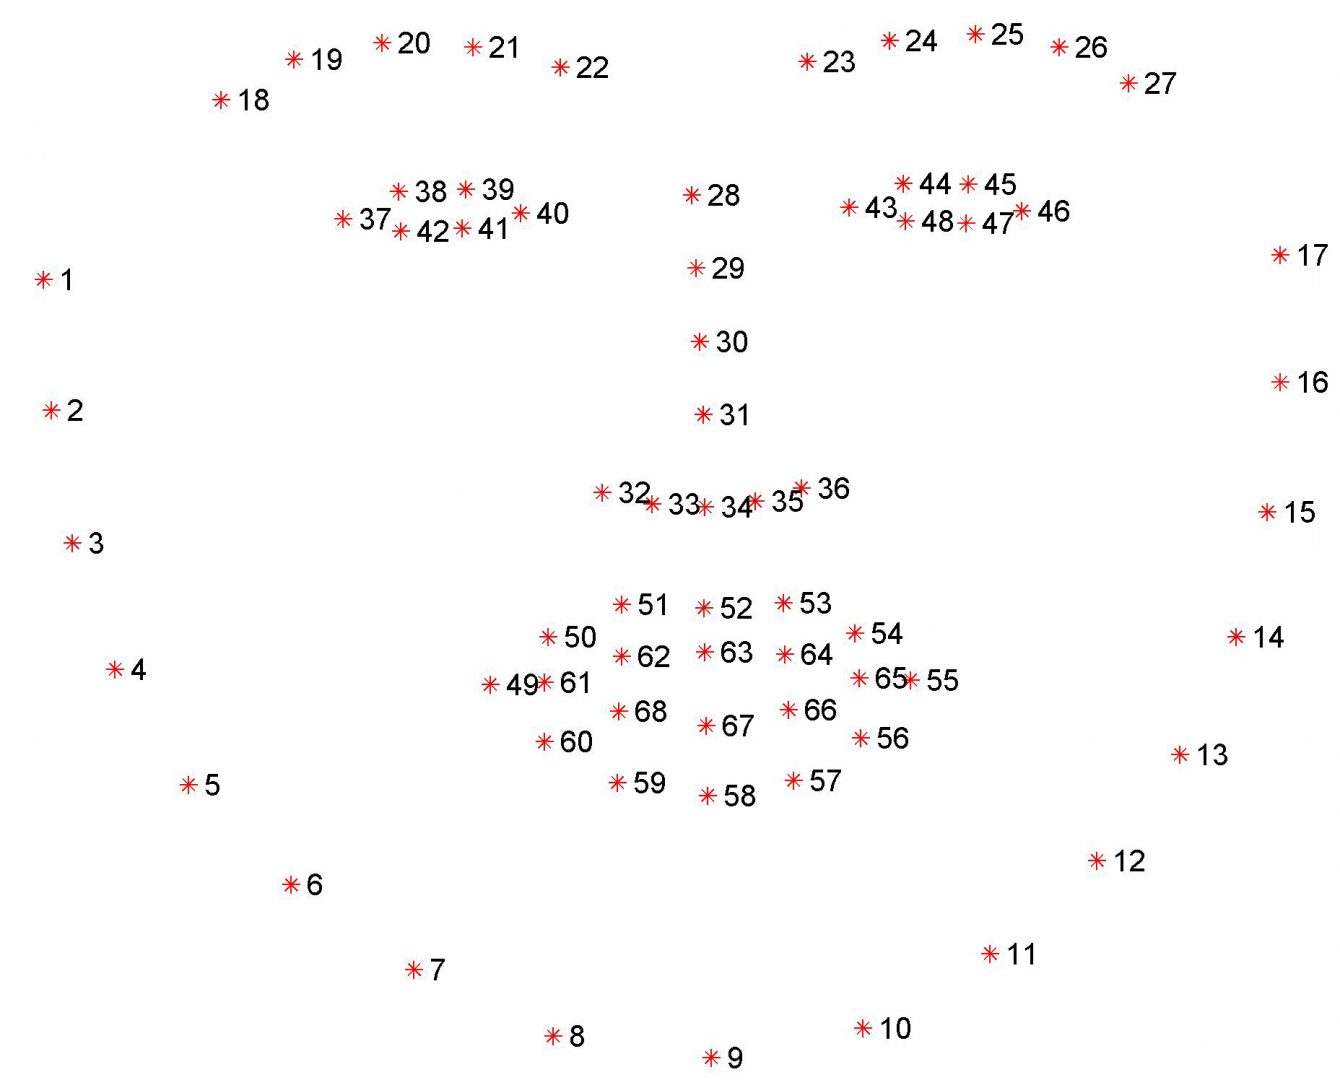
\includegraphics[width=0.2\textwidth]{facial_landmarks.jpg}
    \caption{Dlib facial landmarks.}
    \label{fig:my_label}
\end{figure}
Finally, we used \textbf{dlib}'s facial landmarks recognition free library as it provided 68 points which are enough to crop the mouth from the image smoothly, and detect the facial midline points.
\begin{figure}[H]
   \centering
   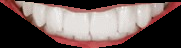
\includegraphics[width=0.2\textwidth]{cropped_mouth.png}
   \caption{Cropped mouth.}
   \label{fig:my_label}
\end{figure}
\subsection{Discolortion}
 The first thing that people notice in someone's smile are the color of their teeth, so, it is very important to detect whether someone's teeth have any discoloration.
 We've successfully detected teeth discoloration by adding a color mask to the cropped mouth image to separate the teeth from the rest of the mouth.
 Then, we've iterated on every pixel in the mask and compared it to a certain range of teeth shades values and detected whether it falls within that range or not.
 Afterwards, we removed the black pixels from the masked image to get rid of any noise that may affect our calculations. Finally, We've counted every pixel that doesn't fall within the predetermined discoloration shades and divided it by the total number of the teeth pixels.
 \begin{figure}[H]
    \centering
    
\includegraphics[width=0.2\textwidth]{segmented_teeth.png}
    \caption{Color segmented teeth.}
    \label{fig:my_label}
\end{figure}
\subsection{Midline Shift}
The position of the mid-line between the central incisors should be on a line drawn from between the eyes anddown through the nose, lips and chin.
After detecting the horizontal position of the facial midline, we started to move horizontally along the mouth from its center in both directions till the two edges of the mouth.
Then, we store and sort every pixel in the way and sort it in an ascending order according to its B component intensity in the BGR color mode.
Next, we select the first 3 pixels with the least blue intensity and calculate the distance between each one of them.
If the distance between the two pixels is less than a certain threshold, we choose the intermediate pixel as the horizontal position of the dental midline.
However, if the distances are not equal, we choose the pixel farest pixel from the center of the mouth. 
\begin{figure}[H]
    \centering
    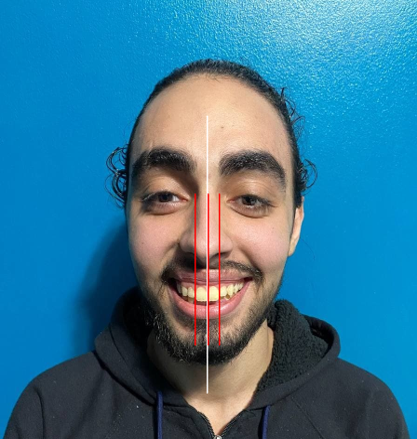
\includegraphics[width=0.3\textwidth]{midline_shift.png}
    \caption{White line is the facial midline and the dental midline is calculated through the 3 red lines.}
    \label{fig:my_label}
\end{figure}
\subsection{Gummy Smile}
A “gummy smile” is when too much gum tissue shows above your front teeth when you smile.
We've detected whether a person smile is a gummy smile or not by calculating the ratio between the gum and the teeth.
The gum is calculated by iterating over the cropped mouth image and getting the number of the pixels that contain gum. Then, this number is divided by the number of teeth pixels.
\begin{figure}[H]
    \centering
    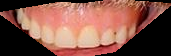
\includegraphics[width=0.2\textwidth]{gummy_smile.png}
    \caption{An example of a gummy smile.}
    \label{fig:my_label}
\end{figure}
\subsection{Diastema}
A "Diastema" is a gap between the central incisors. 
This gap can be detected by converting the cropped image to the grey scale color space. Using canny's edge detection, we can detect the lower edge of the central incisors. 
Then, we move along the vertical line starting from
the lower edge of the central incisors. After that, we move horizontally from the
mouth’s center and count how many dark pixels along the way.
The previous step is repeated along multiple rows of pixels. If
the number of rows passed a certain threshold, then the person
has a disatema
\begin{figure}[H]
    \centering
    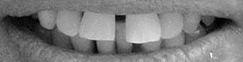
\includegraphics[width=0.2\textwidth]{diastemapng.png}
    \caption{An example of a gummy smile.}
    \label{fig:my_label}
\end{figure}
\subsection{Teeth Coloring}
If the software detected that there's a discoloration, a drop list appears in the UI for the user to select between 2 shades (A1 and B1).
After the user selects the desired shade, a mask with the same color is added to the cropped mouth image to color the teeth and preview it in the UI after adding it. 
\begin{figure}[H]
    \centering
    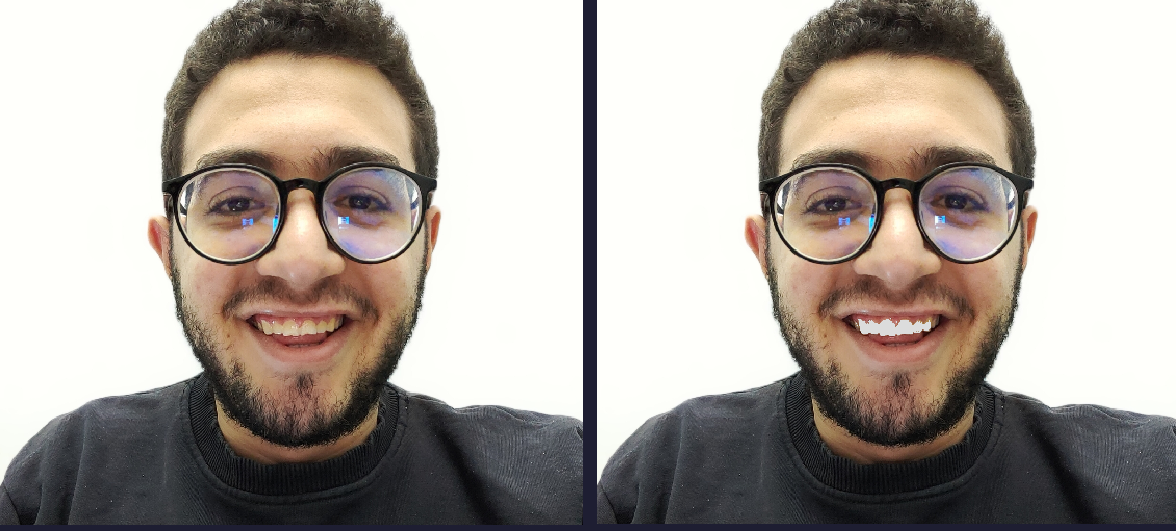
\includegraphics[width=0.6\textwidth]{coloring.png}
    \caption{A before and after image as shown in the GUI.}
    \label{fig:my_label}
\end{figure}
\subsection{Detect Teeth Color}
The software can also detect the mean color of the teeth and match it with a tooth color chart.
\begin{figure}[H]
    \centering
    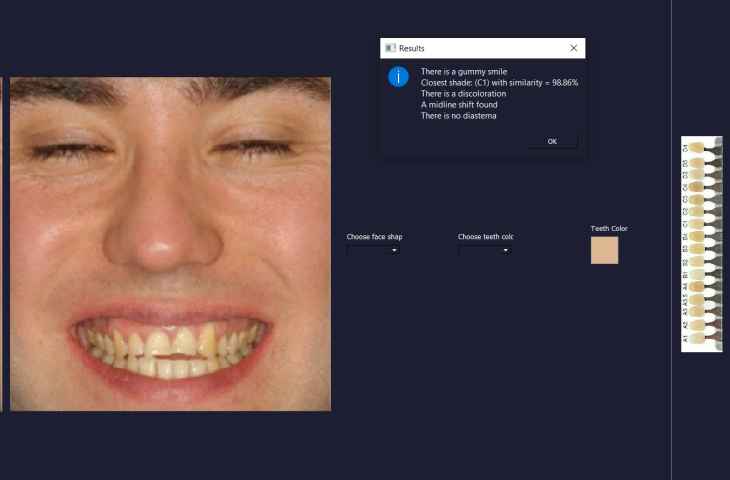
\includegraphics[width=0.5\textwidth]{sahde.png}
    \caption{Teeth color detection.}
    \label{fig:my_label}
\end{figure}
\subsection{Template Matching} 
The user can select between 4 facial structure types and according to it, the softwares applies the corresponding teeth template to the image.
The added template can be moved across the image and resized according to the professional's choice. 
\begin{figure}[H]
    \centering
    
\includegraphics[width=0.5\textwidth]{template.png}
    \caption{Template matching example.}
    \label{fig:my_label}
\end{figure}
\section{\textbf{Results}}

The software was tested on 49 images and had the following results.
\begin{center}
\begin{tabular}{||c c c c||} 
 \hline
 Principle & Successful cases & Accuracy \\ [0.5ex] 
 \hline\hline
 Gummy Smile & 45 & 91.8\% \\[1ex] 
 \hline
 Teeth Discoloration & 44 & 89.8\% \\[1ex] 
 \hline
 Midline Shift & 41 & 83.7\% \\[1ex] 
 \hline
 Diastema & 45 & 91.8\% \\ [1ex] 
\hline
\end{tabular}
\end{center}
\section{\textbf{Discussion}}
Although the results accuracy is quite good, there are some problems and bugs in the software.
First, if the posture of the person in the image is tilted, the midline detection is affected and often leads to wrong results.\\
Second, if the image is taken under poor lighting conditions or a flash of light reflection on the mouth, it changes the color of the teeth or the gum, which leads to inaccurate gummy smile or discoloration detection.
\\Moreover, if the intermediate space between the two central incisors is large but the lower jaw teeth are behind it, this can lead to an error in the detection of a diastema.
\section{Future Work}
The accuracy of the software can be improved by using advanced and improved algorithms to detect the defects. Furthermore, more features can be added to the software such as:
\begin{enumerate}
    \item Horizontal Plane Detection
    \item Golden Proportion Ratio
    \item Vertical Dimension 
    \item Smile at Rest
\end{enumerate}

\section{Conclusion}
Dentists can use the software to diagnose the mentioned defects and use the solutions that the software offers to fix them. Moreover, anyone can use the software as it is has a very simple UI that can detect all of the mentioned defects with the press of a button.

\end{document}